\documentclass[
	ngerman,
	toc=listof, % Abbildungsverzeichnis sowie Tabellenverzeichnis in das Inhaltsverzeichnis aufnehmen
	toc=bibliography, % Literaturverzeichnis in das Inhaltsverzeichnis aufnehmen
	footnotes=multiple, % Trennen von direkt aufeinander folgenden Fußnoten
	parskip=half, % vertikalen Abstand zwischen Absätzen verwenden anstatt horizontale Einrückung von Folgeabsätzen
	numbers=noendperiod % Den letzten Punkt nach einer Nummerierung entfernen (nach DIN 5008)
]{scrartcl}
\pdfminorversion=5 % erlaubt das Einfügen von pdf-Dateien bis Version 1.7, ohne eine Fehlermeldung zu werfen (keine Garantie für fehlerfreies Einbetten!)
\usepackage[utf8]{inputenc} % muss als erstes eingebunden werden, da Meta/Packages ggfs. Sonderzeichen enthalten

% !TEX root = Projektdokumentation.tex

% Hinweis: der Titel muss zum Inhalt des Projekts passen und den zentralen Inhalt des Projekts deutlich herausstellen
\newcommand{\titel}{Evaluierung von \glqq Icinga 2\grqq{}}
\newcommand{\untertitel}{Open Source Monitoring}
\newcommand{\kompletterTitel}{\titel{} -- \untertitel}

\newcommand{\autorName}{Andreas Germer}
\newcommand{\autorAnschrift}{Hagelbach 9}
\newcommand{\autorOrt}{86316 Bachern}

\newcommand{\betriebLogo}{LogoBetrieb.pdf}
\newcommand{\betriebName}{KUKA AG}
\newcommand{\betriebAnschrift}{Zugspitzstraße 140}
\newcommand{\betriebOrt}{86165 Augsburg}

\newcommand{\ausbildungsberuf}{Fachinformatiker für Systemintegration}
\newcommand{\betreff}{Dokumentation zur betrieblichen Projektarbeit}
\newcommand{\pruefungstermin}{Sommer 2020}
\newcommand{\abgabeOrt}{Augsburg}
\newcommand{\abgabeTermin}{21.05.2020}
 % Metadaten zu diesem Dokument (Autor usw.)
% !TEX root = ../Projektdokumentation.tex

% Anpassung an Landessprache ---------------------------------------------------
\usepackage{babel}

% Umlaute ----------------------------------------------------------------------
%   Umlaute/Sonderzeichen wie äüöß direkt im Quelltext verwenden (CodePage).
%   Erlaubt automatische Trennung von Worten mit Umlauten.
% ------------------------------------------------------------------------------
\usepackage[T1]{fontenc}
\usepackage{textcomp} % Euro-Zeichen etc.

% Schrift ----------------------------------------------------------------------
\usepackage{lmodern} % bessere Fonts
\usepackage{relsize} % Schriftgröße relativ festlegen

% Tabellen ---------------------------------------------------------------------
\PassOptionsToPackage{table}{xcolor}
\usepackage{tabularx}
% für lange Tabellen
\usepackage{longtable}
\usepackage{array}
\usepackage{ragged2e}
\usepackage{lscape}
\newcolumntype{w}[1]{>{\raggedleft\hspace{0pt}}p{#1}} % Spaltendefinition rechtsbündig mit definierter Breite

% Grafiken ---------------------------------------------------------------------
\usepackage[dvips,final]{graphicx} % Einbinden von JPG-Grafiken ermöglichen
\usepackage{graphics} % keepaspectratio
\usepackage{floatflt} % zum Umfließen von Bildern
\graphicspath{{Bilder/}} % hier liegen die Bilder des Dokuments

% Sonstiges --------------------------------------------------------------------
\usepackage[titles]{tocloft} % Inhaltsverzeichnis DIN 5008 gerecht einrücken
\usepackage{amsmath,amsfonts} % Befehle aus AMSTeX für mathematische Symbole
\usepackage{enumitem} % anpassbare Enumerates/Itemizes
\usepackage{xspace} % sorgt dafür, dass Leerzeichen hinter parameterlosen Makros nicht als Makroendezeichen interpretiert werden

\usepackage{makeidx} % für Index-Ausgabe mit \printindex
\usepackage[printonlyused]{acronym} % es werden nur benutzte Definitionen aufgelistet

% Einfache Definition der Zeilenabstände und Seitenränder etc.
\usepackage{setspace}
\usepackage{geometry}

% Symbolverzeichnis
\usepackage[intoc]{nomencl}
\let\abbrev\nomenclature
\renewcommand{\nomname}{Abkürzungsverzeichnis}
\setlength{\nomlabelwidth}{.25\hsize}
\renewcommand{\nomlabel}[1]{#1 \dotfill}
\setlength{\nomitemsep}{-\parsep}

\usepackage{varioref} % Elegantere Verweise. „auf der nächsten Seite“
\usepackage{url} % URL verlinken, lange URLs umbrechen etc.

\usepackage{chngcntr} % fortlaufendes Durchnummerieren der Fußnoten
% \usepackage[perpage]{footmisc} % Alternative: Nummerierung der Fußnoten auf jeder Seite neu

\usepackage{ifthen} % bei der Definition eigener Befehle benötigt
\usepackage{todonotes} % definiert u.a. die Befehle \todo und \listoftodos
\usepackage[square]{natbib} % wichtig für korrekte Zitierweise

% PDF-Optionen -----------------------------------------------------------------
\usepackage{pdfpages}
\pdfminorversion=5 % erlaubt das Einfügen von pdf-Dateien bis Version 1.7, ohne eine Fehlermeldung zu werfen (keine Garantie für fehlerfreies Einbetten!)
\usepackage[
    bookmarks,
    bookmarksnumbered,
    bookmarksopen=true,
    bookmarksopenlevel=1,
    colorlinks=true,
% diese Farbdefinitionen zeichnen Links im PDF farblich aus
    linkcolor=AOBlau, % einfache interne Verknüpfungen
    anchorcolor=AOBlau,% Ankertext
    citecolor=AOBlau, % Verweise auf Literaturverzeichniseinträge im Text
    filecolor=AOBlau, % Verknüpfungen, die lokale Dateien öffnen
    menucolor=AOBlau, % Acrobat-Menüpunkte
    urlcolor=AOBlau,
% diese Farbdefinitionen sollten für den Druck verwendet werden (alles schwarz)
    %linkcolor=black, % einfache interne Verknüpfungen
    %anchorcolor=black, % Ankertext
    %citecolor=black, % Verweise auf Literaturverzeichniseinträge im Text
    %filecolor=black, % Verknüpfungen, die lokale Dateien öffnen
    %menucolor=black, % Acrobat-Menüpunkte
    %urlcolor=black,
%
    %backref, % Quellen werden zurück auf ihre Zitate verlinkt
    pdftex,
    plainpages=false, % zur korrekten Erstellung der Bookmarks
    pdfpagelabels=true, % zur korrekten Erstellung der Bookmarks
    hypertexnames=false, % zur korrekten Erstellung der Bookmarks
    linktocpage % Seitenzahlen anstatt Text im Inhaltsverzeichnis verlinken
]{hyperref}
% Befehle, die Umlaute ausgeben, führen zu Fehlern, wenn sie hyperref als Optionen übergeben werden
\hypersetup{
    pdftitle={\titel -- \untertitel},
    pdfauthor={\autorName},
    pdfcreator={\autorName},
    pdfsubject={\titel -- \untertitel},
    pdfkeywords={\titel -- \untertitel},
}


% zum Einbinden von Programmcode -----------------------------------------------
\usepackage{listings}
\usepackage{xcolor}
\definecolor{hellgelb}{rgb}{1,1,0.9}
\definecolor{colKeys}{rgb}{0,0,1}
\definecolor{colIdentifier}{rgb}{0,0,0}
\definecolor{colComments}{rgb}{0,0.5,0}
\definecolor{colString}{rgb}{1,0,0}
\lstset{
    float=hbp,
	basicstyle=\footnotesize,
    identifierstyle=\color{colIdentifier},
    keywordstyle=\color{colKeys},
    stringstyle=\color{colString},
    commentstyle=\color{colComments},
    backgroundcolor=\color{hellgelb},
    columns=flexible,
    tabsize=2,
    frame=single,
    extendedchars=true,
    showspaces=false,
    showstringspaces=false,
    numbers=left,
    numberstyle=\tiny,
    breaklines=true,
    breakautoindent=true,
	captionpos=b,
}
\lstdefinelanguage{cs}{
	sensitive=false,
	morecomment=[l]{//},
	morecomment=[s]{/*}{*/},
	morestring=[b]",
	morekeywords={
		abstract,event,new,struct,as,explicit,null,switch
		base,extern,object,this,bool,false,operator,throw,
		break,finally,out,true,byte,fixed,override,try,
		case,float,params,typeof,catch,for,private,uint,
		char,foreach,protected,ulong,checked,goto,public,unchecked,
		class,if,readonly,unsafe,const,implicit,ref,ushort,
		continue,in,return,using,decimal,int,sbyte,virtual,
		default,interface,sealed,volatile,delegate,internal,short,void,
		do,is,sizeof,while,double,lock,stackalloc,
		else,long,static,enum,namespace,string},
}
\lstdefinelanguage{natural}{
	sensitive=false,
	morecomment=[l]{/*},
	morestring=[b]",
	morestring=[b]',
	alsodigit={-,*},
	morekeywords={
		DEFINE,DATA,LOCAL,END-DEFINE,WRITE,CALLNAT,PARAMETER,USING,
		IF,NOT,END-IF,ON,*ERROR-NR,ERROR,END-ERROR,ESCAPE,ROUTINE,
		PERFORM,SUBROUTINE,END-SUBROUTINE,CONST,END-FOR,END,FOR,RESIZE,
		ARRAY,TO,BY,VALUE,RESET,COMPRESS,INTO,EQ},
}
\lstdefinelanguage{php}{
	sensitive=false,
	morecomment=[l]{/*},
	morestring=[b]",
	morestring=[b]',
	alsodigit={-,*},
	morekeywords={
		abstract,and,array,as,break,case,catch,cfunction,class,clone,const,
		continue,declare,default,do,else,elseif,enddeclare,endfor,endforeach,
		endif,endswitch,endwhile,extends,final,for,foreach,function,global,
		goto,if,implements,interface,instanceof,namespace,new,old_function,or,
		private,protected,public,static,switch,throw,try,use,var,while,xor
		die,echo,empty,exit,eval,include,include_once,isset,list,require,
		require_once,return,print,unset},
}
 % verwendete Packages
% !TEX root = ../Projektdokumentation.tex

% Seitenränder -----------------------------------------------------------------
\setlength{\topskip}{\ht\strutbox} % behebt Warnung von geometry
\geometry{a4paper,left=20mm,right=20mm,top=23mm,bottom=32mm}

\usepackage[
	automark, % Kapitelangaben in Kopfzeile automatisch erstellen
	headsepline, % Trennlinie unter Kopfzeile
	ilines % Trennlinie linksbündig ausrichten
]{scrpage2}

% Kopf- und Fußzeilen ----------------------------------------------------------
\pagestyle{scrheadings}
% chapterpagestyle gibt es nicht in scrartcl
%\renewcommand{\chapterpagestyle}{scrheadings}
\clearscrheadfoot

% Kopfzeile
\renewcommand{\headfont}{\normalfont} % Schriftform der Kopfzeile
\ihead{\large{\textsc{\titel}}\\ \small{\untertitel} \\[2ex] \textit{\headmark}}
\chead{}
\ohead{\includegraphics[scale=0.5]{\betriebLogo}}
\setlength{\headheight}{15mm} % Höhe der Kopfzeile
%\setheadwidth[0pt]{textwithmarginpar} % Kopfzeile über den Text hinaus verbreitern (falls Logo den Text überdeckt)

% Fußzeile
\ifoot{\autorName}
\cfoot{}
\ofoot{\pagemark}

% Überschriften nach DIN 5008 in einer Fluchtlinie
% ------------------------------------------------------------------------------

% Abstand zwischen Nummerierung und Überschrift definieren
% > Schön wäre hier die dynamische Berechnung des Abstandes in Abhängigkeit
% > der Verschachtelungstiefe des Inhaltsverzeichnisses
\newcommand{\headingSpace}{1.5cm}

% Abschnittsüberschriften im selben Stil wie beim Inhaltsverzeichnis einrücken
\renewcommand*{\othersectionlevelsformat}[3]{
  \makebox[\headingSpace][l]{#3\autodot}
}

% Für die Einrückung wird das Paket tocloft benötigt
%\cftsetindents{chapter}{0.0cm}{\headingSpace}
\cftsetindents{section}{0.0cm}{\headingSpace}
\cftsetindents{subsection}{0.0cm}{\headingSpace}
\cftsetindents{subsubsection}{0.0cm}{\headingSpace}
\cftsetindents{figure}{0.0cm}{\headingSpace}
\cftsetindents{table}{0.0cm}{\headingSpace}


% Allgemeines
% ------------------------------------------------------------------------------

\onehalfspacing % Zeilenabstand 1,5 Zeilen
\frenchspacing % erzeugt ein wenig mehr Platz hinter einem Punkt

% Schusterjungen und Hurenkinder vermeiden
\clubpenalty = 10000
\widowpenalty = 10000
\displaywidowpenalty = 10000

% Quellcode-Ausgabe formatieren
\lstset{numbers=left, numberstyle=\tiny, numbersep=5pt, breaklines=true}
\lstset{emph={square}, emphstyle=\color{red}, emph={[2]root,base}, emphstyle={[2]\color{blue}}}

\counterwithout{footnote}{section} % Fußnoten fortlaufend durchnummerieren
\setcounter{tocdepth}{\subsubsectionlevel} % im Inhaltsverzeichnis werden die Kapitel bis zum Level der subsubsection übernommen
\setcounter{secnumdepth}{\subsubsectionlevel} % Kapitel bis zum Level der subsubsection werden nummeriert

% Aufzählungen anpassen
\renewcommand{\labelenumi}{\arabic{enumi}.}
\renewcommand{\labelenumii}{\arabic{enumi}.\arabic{enumii}.}
\renewcommand{\labelenumiii}{\arabic{enumi}.\arabic{enumii}.\arabic{enumiii}}

% Tabellenfärbung:
\definecolor{heading}{rgb}{0.64,0.78,0.86}
\definecolor{odd}{rgb}{0.9,0.9,0.9}
 % Definitionen zum Aussehen der Seiten
% !TEX root = ../Projektdokumentation.tex

% Abkürzungen, ggfs. mit korrektem Leerraum
\newcommand{\bs}{$\backslash$\xspace}
\newcommand{\bspw}{bspw.\xspace}
\newcommand{\bzw}{bzw.\xspace}
\newcommand{\ca}{ca.\xspace}
\newcommand{\dahe}{\mbox{d.\,h.}\xspace}
\newcommand{\etc}{etc.\xspace}
\newcommand{\eur}[1]{\mbox{#1\,\texteuro}\xspace}
\newcommand{\evtl}{evtl.\xspace}
\newcommand{\ggfs}{ggfs.\xspace}
\newcommand{\Ggfs}{Ggfs.\xspace}
\newcommand{\gqq}[1]{\glqq{}#1\grqq{}}
\newcommand{\inkl}{inkl.\xspace}
\newcommand{\insb}{insb.\xspace}
\newcommand{\ua}{\mbox{u.\,a.}\xspace}
\newcommand{\usw}{usw.\xspace}
\newcommand{\Vgl}{Vgl.\xspace}
\newcommand{\zB}{\mbox{z.\,B.}\xspace}

% Befehle für häufig anfallende Aufgaben
\newcommand{\Abbildung}[1]{\autoref{fig:#1}}
\newcommand{\Anhang}[1]{\appendixname{}~\ref{#1}: \nameref{#1} \vpageref{#1}}
\newcommand{\includegraphicsKeepAspectRatio}[2]{\includegraphics[width=#2\textwidth,height=#2\textheight,keepaspectratio]{#1}}
\newcommand{\Zitat}[2][\empty]{\ifthenelse{\equal{#1}{\empty}}{\citep{#2}}{\citep[#1]{#2}}}
\newcommand{\Autor}[1]{\textsc{#1}} % zum Ausgeben von Autoren
\newcommand{\itemd}[2]{\item{\textbf{#1}}\\{#2}} % erzeugt ein Listenelement mit fetter Überschrift

% fügt Tabellen aus einer TEX-Datei ein
\newcommand{\tabelle}[3] % Parameter: caption, label, file
{\begin{table}[htbp]
\centering
\singlespacing
\input{Tabellen/#3}
\caption{#1}
\label{#2}
\end{table}}

\newcommand{\tabelleAnhang}[1] % Parameter: file
{\begin{center}
\singlespacing
\input{Tabellen/#1}
\end{center}}

% einfaches Wechseln der Schrift, z.B.: \changefont{cmss}{sbc}{n}
\newcommand{\changefont}[3]{\fontfamily{#1} \fontseries{#2} \fontshape{#3} \selectfont}

% Verwendung analog zu \includegraphics
\newlength{\myx} % Variable zum Speichern der Bildbreite
\newlength{\myy} % Variable zum Speichern der Bildhöhe
\newcommand\includegraphicstotab[2][\relax]{%
% Abspeichern der Bildabmessungen
\settowidth{\myx}{\includegraphics[{#1}]{#2}}%
\settoheight{\myy}{\includegraphics[{#1}]{#2}}%
% das eigentliche Einfügen
\parbox[c][1.1\myy][c]{\myx}{%
\includegraphics[{#1}]{#2}}%
}

% Linkfarben
\definecolor{AOBlau}{rgb}{0.64, 0.65, 0.67}

% verschiedene Befehle um Wörter semantisch auszuzeichnen ----------------------
\newcommand{\Index}[2][\empty]{\ifthenelse{\equal{#1}{\empty}}{\index{#2}#2}{\index{#1}#2}}
\newcommand{\Fachbegriff}[2][\empty]{\ifthenelse{\equal{#1}{\empty}}{\textit{\Index{#2}}}{\textit{\Index[#1]{#2}}}}
\newcommand{\NeuerBegriff}[2][\empty]{\ifthenelse{\equal{#1}{\empty}}{\textbf{\Index{#2}}}{\textbf{\Index[#1]{#2}}}}

\newcommand{\Ausgabe}[1]{\texttt{#1}}
\newcommand{\Eingabe}[1]{\texttt{#1}}
\newcommand{\Code}[1]{\texttt{#1}}
\newcommand{\Datei}[1]{\texttt{#1}}

\newcommand{\Assembly}[1]{\textsf{#1}}
\newcommand{\Klasse}[1]{\textsf{#1}}
\newcommand{\Methode}[1]{\textsf{#1}}
\newcommand{\Attribut}[1]{\textsf{#1}}

\newcommand{\Datentyp}[1]{\textsf{#1}}
\newcommand{\XMLElement}[1]{\textsf{#1}}
\newcommand{\Webservice}[1]{\textsf{#1}}

\newcommand{\Refactoring}[1]{\Fachbegriff{#1}}
\newcommand{\CodeSmell}[1]{\Fachbegriff{#1}}
\newcommand{\Metrik}[1]{\Fachbegriff{#1}}
\newcommand{\DesignPattern}[1]{\Fachbegriff{#1}}
 % eigene allgemeine Befehle, die z.B. die Arbeit mit LaTeX erleichtern
% !TEX root = ../Projektdokumentation.tex

% Abkürzungen, ggfs. mit korrektem Leerraum
\newcommand{\bs}{$\backslash$\xspace}
\newcommand{\bspw}{bspw.\xspace}
\newcommand{\bzw}{bzw.\xspace}
\newcommand{\ca}{ca.\xspace}
\newcommand{\dahe}{\mbox{d.\,h.}\xspace}
\newcommand{\etc}{etc.\xspace}
\newcommand{\eur}[1]{\mbox{#1\,\texteuro}\xspace}
\newcommand{\evtl}{evtl.\xspace}
\newcommand{\ggfs}{ggfs.\xspace}
\newcommand{\Ggfs}{Ggfs.\xspace}
\newcommand{\gqq}[1]{\glqq{}#1\grqq{}}
\newcommand{\inkl}{inkl.\xspace}
\newcommand{\insb}{insb.\xspace}
\newcommand{\ua}{\mbox{u.\,a.}\xspace}
\newcommand{\usw}{usw.\xspace}
\newcommand{\Vgl}{Vgl.\xspace}
\newcommand{\zB}{\mbox{z.\,B.}\xspace}

% Befehle für häufig anfallende Aufgaben
\newcommand{\Abbildung}[1]{\autoref{fig:#1}}
\newcommand{\Anhang}[1]{\appendixname{}~\ref{#1}: \nameref{#1} \vpageref{#1}}
\newcommand{\includegraphicsKeepAspectRatio}[2]{\includegraphics[width=#2\textwidth,height=#2\textheight,keepaspectratio]{#1}}
\newcommand{\Zitat}[2][\empty]{\ifthenelse{\equal{#1}{\empty}}{\citep{#2}}{\citep[#1]{#2}}}
\newcommand{\Autor}[1]{\textsc{#1}} % zum Ausgeben von Autoren
\newcommand{\itemd}[2]{\item{\textbf{#1}}\\{#2}} % erzeugt ein Listenelement mit fetter Überschrift

% fügt Tabellen aus einer TEX-Datei ein
\newcommand{\tabelle}[3] % Parameter: caption, label, file
{\begin{table}[htbp]
\centering
\singlespacing
\input{Tabellen/#3}
\caption{#1}
\label{#2}
\end{table}}

\newcommand{\tabelleAnhang}[1] % Parameter: file
{\begin{center}
\singlespacing
\input{Tabellen/#1}
\end{center}}

% einfaches Wechseln der Schrift, z.B.: \changefont{cmss}{sbc}{n}
\newcommand{\changefont}[3]{\fontfamily{#1} \fontseries{#2} \fontshape{#3} \selectfont}

% Verwendung analog zu \includegraphics
\newlength{\myx} % Variable zum Speichern der Bildbreite
\newlength{\myy} % Variable zum Speichern der Bildhöhe
\newcommand\includegraphicstotab[2][\relax]{%
% Abspeichern der Bildabmessungen
\settowidth{\myx}{\includegraphics[{#1}]{#2}}%
\settoheight{\myy}{\includegraphics[{#1}]{#2}}%
% das eigentliche Einfügen
\parbox[c][1.1\myy][c]{\myx}{%
\includegraphics[{#1}]{#2}}%
}

% Linkfarben
\definecolor{AOBlau}{rgb}{0.64, 0.65, 0.67}

% verschiedene Befehle um Wörter semantisch auszuzeichnen ----------------------
\newcommand{\Index}[2][\empty]{\ifthenelse{\equal{#1}{\empty}}{\index{#2}#2}{\index{#1}#2}}
\newcommand{\Fachbegriff}[2][\empty]{\ifthenelse{\equal{#1}{\empty}}{\textit{\Index{#2}}}{\textit{\Index[#1]{#2}}}}
\newcommand{\NeuerBegriff}[2][\empty]{\ifthenelse{\equal{#1}{\empty}}{\textbf{\Index{#2}}}{\textbf{\Index[#1]{#2}}}}

\newcommand{\Ausgabe}[1]{\texttt{#1}}
\newcommand{\Eingabe}[1]{\texttt{#1}}
\newcommand{\Code}[1]{\texttt{#1}}
\newcommand{\Datei}[1]{\texttt{#1}}

\newcommand{\Assembly}[1]{\textsf{#1}}
\newcommand{\Klasse}[1]{\textsf{#1}}
\newcommand{\Methode}[1]{\textsf{#1}}
\newcommand{\Attribut}[1]{\textsf{#1}}

\newcommand{\Datentyp}[1]{\textsf{#1}}
\newcommand{\XMLElement}[1]{\textsf{#1}}
\newcommand{\Webservice}[1]{\textsf{#1}}

\newcommand{\Refactoring}[1]{\Fachbegriff{#1}}
\newcommand{\CodeSmell}[1]{\Fachbegriff{#1}}
\newcommand{\Metrik}[1]{\Fachbegriff{#1}}
\newcommand{\DesignPattern}[1]{\Fachbegriff{#1}}
 % eigene projektspezifische Befehle, z.B. Abkürzungen usw.

\begin{document}

\phantomsection
\thispagestyle{plain}
\pdfbookmark[1]{Deckblatt}{deckblatt}
% !TEX root = Projektdokumentation.tex
\begin{titlepage}

\begin{center}

\includegraphics[scale=0.25]{LogoIHK.pdf}\\[1ex]
\Large{Abschlussprüfung \pruefungstermin}\\[3ex]

\Large{\ausbildungsberuf}\\
\LARGE{\betreff}\\[4ex]

\huge{\textbf{\titel}}\\[1.5ex]
\Large{\textbf{\untertitel}}\\[4ex]

\normalsize
Abgabetermin: \abgabeOrt, den \abgabeTermin\\[3em]
\textbf{Prüfungsbewerber:}\\
\autorName\\
\autorAnschrift\\
\autorOrt\\[5ex]

\includegraphics[scale=1]{\betriebLogo}\\[2ex]
\textbf{Ausbildungsbetrieb:}\\
\betriebName\\
\betriebAnschrift\\
\betriebOrt\\[5em]
\end{center}

\small
\noindent
Dieses Werk einschließlich seiner Teile ist \textbf{urheberrechtlich geschützt}.
Jede Verwertung außerhalb der engen Grenzen des Urheberrechtgesetzes ist ohne
Zustimmung des Autors unzulässig und strafbar. Das gilt insbesondere für
Vervielfältigungen, Übersetzungen, Mikroverfilmungen sowie die Einspeicherung
und Verarbeitung in elektronischen Systemen.

\end{titlepage}
\cleardoublepage

% Preface --------------------------------------------------------------------
\phantomsection
\pagenumbering{Roman}
\pdfbookmark[1]{Inhaltsverzeichnis}{inhalt}
\tableofcontents
\cleardoublepage

\phantomsection
\listoffigures
\cleardoublepage

\phantomsection
\listoftables
\cleardoublepage

\phantomsection
\lstlistoflistings
\cleardoublepage

\newcommand{\abkvz}{Abkürzungsverzeichnis}
\renewcommand{\nomname}{\abkvz}
\section*{\abkvz}
\markboth{\abkvz}{\abkvz}
\addcontentsline{toc}{section}{\abkvz}
% !TEX root = Projektdokumentation.tex

% Es werden nur die Abkürzungen aufgelistet, die mit \ac definiert und auch benutzt wurden. 
%
% \acro{VERSIS}{Versicherungsinformationssystem\acroextra{ (Bestandsführungssystem)}}
% Ergibt in der Liste: VERSIS Versicherungsinformationssystem (Bestandsführungssystem)
% Im Text aber: \ac{VERSIS} -> Versicherungsinformationssystem (VERSIS)

% Hinweis: allgemein bekannte Abkürzungen wie z.B. bzw. u.a. müssen nicht ins Abkürzungsverzeichnis aufgenommen werden
% Hinweis: allgemein bekannte IT-Begriffe wie Datenbank oder Programmiersprache müssen nicht erläutert werden,
%          aber ggfs. Fachbegriffe aus der Domäne des Prüflings (z.B. Versicherung)

% Die Option (in den eckigen Klammern) enthält das längste Label oder
% einen Platzhalter der die Breite der linken Spalte bestimmt.
\begin{acronym}[WWWW]
	\acro{PHP}{Hypertext Preprocessor; Skriptsprache zur Erstellung von Websites}
	\acro{CPU}{Central Processing Unit; Hauptprozessor}
	\acro{RAM}{Random-Access Memory; Arbeitsspeicher}
	\acro{VM}{Virtuelle Maschine}
	\acro{LAN}{Local Area Network}
	\acro{LDAP}{Lightweight Directory Access Protocol; Protokoll zur Abfrage von Verzeichnisdiensten}
	\acro{FQDN}{Full Qualified Domain Name; eindeutige Adresse eines Hosts im Netzwerk}
	\acro{HTTP}{Hypertext Transfer Protocol; Protokoll zur Übertragung von z.B. Websites}
	\acro{URL}{Uniform Resource Locator; hier: Internetadresse}
	\acro{ESXi}{Typ-1 Hypervisor von VMware}
	\acro{ISO}{Speicherabbild eines Dateisystems}
\end{acronym}

\clearpage

% Inhalt ---------------------------------------------------------------------
\pagenumbering{arabic}
% !TEX root = Projektdokumentation.tex
% !TEX root = ../Projektdokumentation.tex
\section{Einleitung}
\label{sec:Einleitung}

\subsection{Projektumfeld} 
\label{sec:Projektumfeld}
Die KUKA AG ist ein international tätiges Unternehmen in der Maschinenbau- und Automatisierungsbranche mit rund 14.200 Mitarbeitern. Zum Produktportfolio zählen neben Industrierobotern auch die Planung und der Bau von Produktionsstraßen.

Die IT-Infrastruktur am Standort Augsburg besteht aus ca. 1.200 größtenteils virtualisierten Servern; an anderen Standorten befindet sich vereinzelt eine kleine Anzahl an Servern. Es kommen alle gängigen Betriebssysteme zum Einsatz. Auftraggeber dieses Projekts ist die Abteilung \glqq Datacenter \& Network\grqq{}, die den Betrieb der Rechenzentren sowie des internen IT-Netzwerks der KUKA AG überwacht und koordiniert.

\subsection{Projektziel} 
\label{sec:Projektziel}
Momentan wird kein einheitliches Monitoring der IT-Systeme durchgeführt. Die verschiedenen Standorte und Abteilungen setzen auf unterschiedliche und teils veraltete Lösungen; zur besseren Administration sollen diese durch ein einheitliches und zentrales System ersetzt werden.

Es soll evaluiert werden, ob die freie Monitoringsoftware \glqq Icinga\grqq{} für firmeninternen Einsatz geeignet ist. Dazu werden in einem ersten Schritt Anforderungen der Process Owner und Systemadministratoren gesammelt. Anschließend wird eine Testumgebung eingerichtet, um zu prüfen, inwieweit die Ansprüche des Unternehmens durch \glqq Icinga\grqq{} erfüllt werden können. Abschließend werden die Ergebnisse analysiert und eine Empfehlung ausgesprochen.

\subsection{Projektbegründung} 
\label{sec:Projektbegruendung}
Durch die zunehmende Digitalisierung aller Geschäftsprozesse sind Unternehmen äußerst abhängig von Computersystemen. Wird das Schutzziel der Verfügbarkeit nicht ausreichend gut verfolgt, kommt es zu Systemausfällen und der Geschäftsbetrieb ist nicht mehr möglich - mit unabsehbaren wirtschaftlichen Folgen. Um Ausfallsicherheit zu gewährleisten, ist ein umfangreiches und zuverlässiges Monitoring aller Ressourcen unerlässlich.

\subsection{Projektabgrenzung} 
\label{sec:Projektabgrenzung}
Als Monitoringsystem interagiert \glqq Icinga\grqq{} potenziell mit allen Geräten und Diensten im Netzwerk. Für dieses Projekt wird das Zusammenspiel auf virtuelle Maschinen mit ausgewählten Betriebssystemen und Diensten eingegrenzt.
% !TEX root = ../Projektdokumentation.tex
\section{Projektplanung} 
\label{sec:Projektplanung}

\subsection{Projektphasen}
\label{sec:Projektphasen}
Das Projekt wird innerhalb einer 35-Stunden-Arbeitswoche durchgeführt. Die einzelnen Phasen werden sich teils überschneiden; beispielsweise können virtuelle Maschinen bereits eingerichtet werden, während noch auf Rückmeldungen bezüglich der Anforderungen an das System gewartet wird. 
\tabelle{Zeitplanung}{tab:Zeitplanung}{ZeitplanungKurz}

\subsection{Abweichungen vom Projektantrag}
\label{sec:AbweichungenProjektantrag}
Es gab keine Abweichungen vom Projektantrag.

\subsection{Ressourcenplanung}
\label{sec:Ressourcenplanung}
Folgende Hardware wird zur Durchführung des Projekts benötigt:
\begin{itemize}
  \item Notebook mit RJ-45 Port und USB Port
  \item Workstation mit mindestens: 2x RJ-45 Port, 2x USB Port, 16 GB Arbeitsspeicher, 500 GB HDD
  \item Software: Windows 10 (min. Professional), Windows Server (min. 2012), Debian (aktuelle Version), Ubuntu (aktuelle Version), ESXi (aktuelle Version), aktueller Webbrowser, SSH-Client
  \item 2x Netzwerkkabel, min. 1,5m
  \item USB-Datenträger, 8GB
\end{itemize}
% !TEX root = ../Projektdokumentation.tex
\section{Planungsphase} 
\label{sec:Planungsphase}

\subsection{Ist-Analyse} 
\label{sec:IstAnalyse}
Zu Projektbeginn existiert im Unternehmen keine einheitliche Lösung zur Serverüberwachung. Für den Großteil der Server am Standort Augsburg wird der \glqq Advanced Host Monitor\grqq{} eingesetzt. Diese Lösung erhält trotz ihres Alters noch regelmäßige Updates, aufgrund eines veralteten User Interfaces, einem beschränktem Funktionsumfang sowie der nicht mehr ausreichenden Leistungsfähigkeit, wird seit mehreren Jahren der Wunsch nach einem neuen Monitoring-System geäußert.

Die Entwicklungsabteilungen überwachen die von ihnen betreuten Server mit einer auf \glqq Elasticsearch\grqq{} und \glqq Kibana\grqq{} basierenden Lösung. Um Know-how zu bündeln und Personalkosten zu sparen, signalisierten die Verantwortlichen eine Bereitschaft zur Zusammenlegung des Servermonitoring.

Am Standort Bremen wird seit mehreren Jahren auf die Open-Source-Anwendung \glqq Icinga\grqq{} gesetzt. Die Systembetreuenden haben mit dieser Lösung positive Erfahrungen gemacht, und loben insbesondere die einfache Erweiterbarkeit durch Plugins, sowie die Möglichkeit ohne Aufwand optisch ansprechende Dashboards zu erstellen. Aufgrund der Komplexität dieser Software und einem anstehenden Update auf \glqq Icinga 2\grqq{} wurde auch von dieser Seite der Wunsch nach einem einheitlichen und zentral verwaltetem Servermonitoring geäußert.

\subsection{Soll-Analyse} 
\label{sec:SollAnalyse}

\subsubsection{Befragung der Fachabteilungen}
\label{sec:BefragungFachabteilungen}
Es wurden die entsprechenden Verantwortlichen via E-Mail, Telefonaten und Meetings zu den betreuten Servern und deren Monitoring befragt. Hierbei zeigten sich große Überschneidungen bei den Serverumgebungen sowie den Anforderungen an deren Überwachung, was eine Zusammenlegung logisch erscheinen lässt.

Über alle Abteilungen hinweg werden verschiedenste Windows-Versionen sowie Linux-Distributionen eingesetzt, weswegen ausschließlich ein plattformunabhängiges Monitoring-System wie \glqq Icinga 2\grqq{} eingesetzt werden kann. Die zu überwachenden Parameter beziehungsweise Dienste ähneln sich zwischen den Abteilungen ebenfalls sehr stark: Neben Leistungsmetriken wie Prozessorauslastung, Arbeitsspeicherbelegung oder freiem Massenspeicher wird viel Wert auf die Überprüfung der Erreichbarkeit im Netzwerk gelegt. Aufgrund der zunehmenden Verbreitung von webbasierten Anwendungen soll auch der Betrieb von Webservern überwacht werden. Weiterhin wurde der Wunsch nach einer ansprechenden grafischen Aufbereitung geäußert.

\subsubsection{Kriterienkatalog}
\label{sec:Kriterienkatalog}
Auf Basis der Befragungen wurde folgender Kriterienkatalog aufgestellt:
\begin{itemize}
	\item Überwachbare Betriebssysteme: Alle gängigen Windows Server Versionen und Linux-Distributionen
	\item Überwachbare Systemparameter: CPU-Auslastung, RAM-Belegung, Massenspeicherbelegung
	\item Überwachung von Webservern
	\item Ansprechende und anpassbare grafische Aufbereitung
\end{itemize}

\subsection{Wirtschaftlichkeitsanalyse}
\label{sec:Wirtschaftlichkeitsanalyse}

\subsubsection{Projektkosten}
\label{sec:Projektkosten}
Die Kosten, die durch das Projekt verursacht werden, setzen sich sowohl aus Personal- als auch aus Ressourcenkosten zusammen. Die Berechnung der Stundensätze findet sich im \Anhang{app:Stundensatz}.

Die Kosten für die 35-Stunden-Woche des Auszubildenden belaufen sich auf \eur{350}. Die Arbeitszeit, die bei mitarbeitenden Personen zur Durchführung des Projekts angefallen ist (z.B. für Befragungen, Konfiguration der Netzwerkkomponenten, Anpassungen der Firewall für Updates, Abnahme) wurde auf vier Stunden geschätzt. Dafür fielen also Personalkosten in Höhe von \eur{160} an. Die für das Projekt eingesetzte Hardware ist bereits abgeschrieben, und wird mit einer Pauschale von \eur{360} pro Jahr verrechnet. Auf die Projektdauer von fünf Tagen ergibt das Betriebskosten von \eur{4,93}.

Eine Aufstellung der Projektosten befindet sich in Tabelle~\ref{tab:Kostenaufstellung}. Sie betragen insgesamt \eur{514,93}.
\tabelle{Kostenaufstellung Projekt}{tab:Kostenaufstellung}{Kostenaufstellung.tex}

\subsubsection{Betriebskosten des Monitorings}
\label{sec:BetriebskostenMonitoring}
Die Betriebskosten für ein Monitoringsystem umfassen Personalkosten für Wartungsarbeiten und Anpassungen, sowie die Kosten die für zwei redundant ausgelegte Hardware-Server anfallen. Diese werden benötigt, da das Monitoring nicht innerhalb der Virtualisierungsumgebung betrieben werden sollte, um eine funktionierende Serverüberwachung auch bei Ausfall der VM-Infrastruktur zu gewährleisten.

Für das Einpflegen neuer Server oder Funktionen wird eine Arbeitsstunde pro Woche veranschlagt. Weiterhin wird der Arbeitsaufwand für Updates und Fehlerbehebungen nach Erfahrungsberichten auf acht Stunden pro Quartal geschätzt. Auf ein Jahr summiert ergibt beides einen Arbeitsaufwand von insgesamt 84 Stunden.

Die geschätzten Kosten für einen Hardware-Server belaufen sich auf \eur{4.000} jährlich. Die Gesamtkosten für den Betrieb einer Monitoring-Instanz belaufen sich, wie in Tabelle~\ref{tab:Monitoringkosten} dargelegt, auf \eur{11.360,00} pro Jahr.
\tabelle{Kostenaufstellung Monitoring}{tab:Monitoringkosten}{Monitoringkosten.tex}

\subsubsection{Amortisationsdauer}
\label{sec:Amortisationsdauer}
Sollte die Evaluation durch diese Projektarbeit ergeben, dass \glqq{}Icinga 2\grqq{} für den firmenweiten Einsatz geeignet ist, werden drei momentan im Betrieb befindliche Monitoringinstanzen (siehe \ref{sec:IstAnalyse} \nameref{sec:IstAnalyse}) durch ein zentrales \glqq{}Icinga 2\grqq{}-System ersetzt (siehe \ref{sec:Projektziel} \nameref{sec:Projektziel}). Die Betriebskosten für die derzeitigen Überwachungssysteme entsprechen etwa den in \ref{sec:BetriebskostenMonitoring} \nameref{sec:BetriebskostenMonitoring} berechneten \eur{11.360,00} pro Jahr; die jährliche Einsparung, wenn statt drei Systemen nur noch eines betrieben wird, beläuft sich also auf:
\begin{eqnarray}
\eur{11.360,00} \cdot 2 = \eur{22.720,00}
\end{eqnarray}
Für die Ersteinrichtung des neuen Systems werden etwa zwei Wochen benötigt, also insgesamt 70 Arbeitsstunden. Das verursacht einmalige Kosten in Höhe von:
\begin{eqnarray}
70 \mbox{h} \cdot \eur{40,00} \mbox{/h} = \eur{2.800}
\end{eqnarray}
Die Amortisationszeit beträgt also:
\begin{eqnarray}
\frac{\eur{2.800}}{\eur{22.720,00}\mbox{/a}} \approx 0,123 \mbox{ Jahre} \approx 45 \mbox{ Tage}
\end{eqnarray}
\setcounter{equation}{0}
% !TEX root = ../Projektdokumentation.tex
\section{Durchführungsphase}
\label{sec:Durchführungsphase}

\subsection{Vorbereitung der Tests}
\label{sec:VorbereitungTests}

\subsubsection{Vorbereiten der Hardware}
\label{sec:VorbereitungHardware}
Eine ausrangierte DELL Precision Workstation dient als Hardwareplattform für das Projekt. Die Ausstattung von 32 Gigabyte Arbeitsspeicher und einem Intel Xeon Hochleistungsprozessor ist ausreichend für den Betrieb von mehreren virtuellen Maschinen.

Um den Bedingungen in einem \glqq{}echtem\grqq{} Rechencenter möglichst nahe zu kommen, wird der VM-Hypervisor mit zwei Netzwerkschnittstellen ausgestattet. Ein Interface ist für die Kommunikation mit dem Hypervisor selbst vorgesehen (sogenanntes Management-LAN), und eine weitere Netzwerkschnittstelle wird von den virtuellen Maschinen benutzt, um im Netzwerk erreichbar zu sein. Da die Workstation nur über einen Netzwekport verfügte, musste eine zweite Netzwerkkarte eingebaut werden.

\subsubsection{Installation des Hypervisors}
\label{sec:InstallationHypervisor}
Um die gegeben Ressourcen optimal auszunutzen, wird ein sogenannter Typ 1-Hypervisor eingesetzt. Dieser kommuniziert direkt mit der Hardware, ohne dass ein anderes Betriebssystem zum Einsatz kommt. Für dieses Projekt wird das System \glqq{}ESXi\grqq{} von VMware in der Version 6.7 verwendet, das auch in den firmeneigenen Rechenzentren zum Einsatz kommt.

Die Installation gestaltet sich als simpel. Nachdem wichtige UEFI-Optionen angepasst wurden (UEFI statt legacy-BIOS; hardewareseitige Virtualisierungsunterstützung) wird das System von einem USB-Datenträger, der zuvor mit dem ESXi-Image geflasht wurde, gestartet. Nachdem die für die Installation zu benutzende Festplatte ausgewählt, und ein Root-Passwort vergeben wurde, startet der Installationsvorgang. Nach abgeschlossener Installation muss noch eine IP-Adresse für das Managementnetzwerk vergeben werden.

Die restliche Konfiguration geschieht bequem über eine Weboberfläche. Der Lizenzschlüssel wird hinterlegt, die zweite Festplatte als Datastore eingebunden, und das Netzwerk für die virtuellen Maschinen konfiguriert (siehe Abbildung \ref{screen:vmnetwork}). Hierzu wird ein neuer virtueller Switch für den zweiten Netzwerkport (der, der nicht mit dem Management-LAN belegt ist) erstellt und mit einer neuen Port Group versehen. Diese Port Groups werden in ESXi verwendet, um logische Netzwerkschnittstellen bereit zu stellen und zu verwalten. 

\subsubsection{Installation der virtuellen Maschinen}
\label{sec:InstallationVMs}
Für virtuelle Maschinen muss in der ESXi-Weboberfläche zunächst die Systemkonfiguration festgelegt werden. Hierfür werden die für die VM vorgesehene CPU-Kerne, Arbeits- und Massenspeicherspeicherkapazität (siehe Abbildung \ref{screen:vmcreation}) sowie die zu benutzenden Port Groups eingestellt. Abschließend wird in ein virtuelles DVD-Laufwerk das ISO-Abbild für das entsprechende zu installierende Betriebssystem eingehängt, und die virtuelle Maschine gestartet. Die anschließende Betriebssysteminstallation kann über eine emulierte Browser-Konsole durchgeführt werden.

Um in diesem Testsystem eine möglichst nah an das Firmennetzwerk heranzukommen, wurden drei Betriebssysteme für die Server ausgewählt: Windows Server 2019, Ubuntu 18.04 LTS sowie Debian 10.3. Die Installation der Systeme verlief ohne Probleme.

\subsubsection{Installation von \glqq{}Icinga\grqq{}}
\label{sec:InstallationIcinga}
Die Installation von \glqq{}Icinga\grqq{} unter Ubuntu beginnt mit dem Aufruf der Rootshell und einem anschließendem kompletten Systemupdate. Die Pakete \code{icinga2} und \code{icingacli} sind für die Monitoring-Engine an sich sowie die Verwaltung über Kommandozeile zuständig und können über die Paketverwaltung installiert werden. \code{monitoring-plugins} installiert Plugins für die wichtigsten Monitoringaufgaben (z.B. Ping).
\footnote{Eine komplette (nachträglich optimierte) Liste an Befehlen, die für eine komplette Installation unter Ubuntu 18.04 ausgeführt werden muss, findet sich im \Anhang{app:skript}}

Aufgrund der firmeninteren Verbreitung sowie der In-Memory Unterstützung wird MySQL als Datenbanksystem verwendet. Durch Installation der Pakete \code{mysql-server} und \code{mysql-client} werden ein MySQL-Server und ein MySQL-Client bereitgestellt, das Skript \code{mysql\_{}secure\_{}installation} (siehe Abbildung \ref{screen:mysqlsecure}) verbessert die Sicherheit durch Maßnahmen wie das Entfernen von anonymen Accounts oder die Absicherung des root-Accounts.

Im nächsten Schritt muss die Schnittstelle zwischen \glqq{}Icinga Data Output\grqq{} (Exportfunktion für Monitoringdaten; kurz IDO) und MySQL geschaffen werden, damit die gesammelten Daten auch gespeichert werden können. Dies geschieht durch Installation des Pakets \code{icinga2-ido-mysql}. Anschließend kann das Webinterface \code{icingaweb2} installiert werden.

Beim Versuch, das Web-Frontend aufzurufen, wird lediglich ein PHP-Fehler angezeigt. Es ergab sich, dass dieser Fehler durch Inkompatibilitäten mit bestimmten PHP 7.2 Plugins verursacht wird. Dieser Fehler wurde bereits Mitte 2018 behoben, allerdings ist der Bugfix anscheinend nicht in das Paket eingespielt worden. Das Problem wurde gelöst, indem die aktuelle Version von \glqq{}Icinga Web 2\grqq{} vom öffentlichen Github-Repository nach \code{/usr/share/icingaweb2} geklont wurde.

Ist \glqq{}Icinga Web 2\grqq{} fertig installiert, muss noch ein Benutzer für die MySQL-Datenbank erstellt werden. Abschließend wird IDO mittels \code{icinga2 feature enable command ido-mysql} aktiviert, und ein Setup-Token mit \code{icingacli setup token create} generiert werden. Nach einem Neustart des icinga2-Dienstes (\code{systemctl restart icinga2}) ist \glqq{}Icinga 2\grqq{} bereit über eingerichtet zu werden.

\paragraph{Einrichtung über Webfrontend}
Im Browser wird nun (IP-Adresse des Servers)/icingaweb2/setup aufgerufen, um den Konfigurationsassistenten (siehe Abbildung \ref{screen:konfigassistent}) zu starten. Nach Eingabe des vorher generierten Setup-Tokens wird im ersten Schritt geprüft, ob alle notwendigen PHP-Plugins vorhanden sind. In der für diese Projekt durchgeführten Installation fehlten die Plugins \glqq{}PDO-PostgreSQL\grqq{}, welches aufgrund der Verwendung von MySQL nicht benötigt wird, sowie \glqq{}cURL\grqq{}, das mittels \code{apt install php7.2-curl} nachinstalliert wurde.

Im Abschnitt \glqq{}Configuration\grqq{} werden noch kleinere, weitere Einstellungen getroffen, hierbei bietet sich aber an, die Standardeinstellungen beizubehalten. Eine Ausnahme stellt die bevorzugte Authentifizierungsmethode für Nutzende des Frontends dar; hier kann zwischen LDAP und einer Datenbank mit Benutzern gewählt werden. Für dieses Projekt wurde aufgrund des geringeren Umfangs letztere Option gewählt, die Konfiguration hierfür findet sich in Abbildung \ref{screen:userdb}.

\paragraph{Einpflegen von Servern}
Durch Installation des Plugins \glqq{}Icinga Director\grqq{} kann das Hinzufügen von zu überwachenden Server über die Webschnittstelle erledigt werden; für dieses Projekt wird darauf verzichtet und die weitergehende Konfiguration geschieht über Anpassung der Konfigurationsdateien unter \code{/etc/icinga2/conf.d/}. Dort können in der Datei \code{hosts.conf} neue Server hinzugefügt werden (siehe Abbildung \ref{screen:newservers}). Abschließend kann die Syntax der Konfigurationsdateien mittels \code{icinga2 daemon --validate} überprüft werden; nach einem Neustart des \glqq{}Icinga 2\grqq{} Dienstes sind die neuen Hosts im Monitoring verfügbar.

\paragraph{Installation des Agents}
Mit der bisherigen Konfiguration können einfache Checks (z.B. Ping) auf die entsprechenden Hosts durchgeführt werden. Für aufwendigere Überprüfungen wie Speicherplatzkontrolle muss auf den Hosts eine Software installiert werden. Hierfür muss zunächst der Monitoringserver als \glqq{}Master\grqq{} deklariert werden, dies geschieht mittels des Befehls \code{icinga2 node wizard}. Anschließend wird mit \code{sudo icinga2 pki ticket --cn (FQDN)} noch ein \glqq{}Ticket\grqq{} für den angegebenen FQDN erstellt, mithilfe dessen der Host die Verbindung zum Master herstellen kann.

Der Host selbst installiert die Software ebenfalls, auf Linux-basierten Systemen besteht dies einfach aus dem Paket \code{icinga2}, für Windows existieren herunterladbare Installationsdateien. Mit Durchführung des Befehls \code{icinga2 node wizard} wird die Konfiguration des Agents abgeschlossen, bei Windows geschieht dies über ein grafisches Userinterface. Nachdem die Adresse des Masters sowie die eben erstellte Ticketnummer angegeben und eventuell Ports angepasst wurden, stellt der Agent eine Verbindung zum Monitoring her.

\subsection{Durchführung der Tests}
\label{sec:DurchführungTests}

\subsubsection{Betriebssystemkompatibilität}
\label{sec:oscompatibility}
Es konnten keine Probleme bei der Integration von anderen Betriebsystemen festgestellt werden. Sowohl unter Ubuntu 18.04, Debian 10 und Windows Server 1809 läuft \glqq{}Icinga 2\grqq{} ohne Probleme. Eine umfassende Betriebssystemkompatibilität ist somit gewährleistet.

\subsubsection{Überwachung von Leistungsparametern}
\label{sec:ÜberwachungLeistungsparameter}
Das installierte Pluginpaket \code{monitoring-plugins} beinhaltet Plugins zur Überwachung der Leistungsparametern (CPU-Auslastung, RAM-Belegung und belegter Massenspeicher). Für diese Überprüfungen müssen in \code{/etc/icinga2/conf.d/commands.conf} Definitionen erstellt werden. Am Beispiel in Abbildung \ref{screen:loaddefinition} ist erkenntlich, dass diese Definitionen neben dem auszuführendem Befehl (diese sind als Bash-Skript abgelegt; das Verzeichnis hierfür ist in der Konstante \glqq{}PluginDir\grqq{} gespeichert) auch die zu übergebenden Argumente enthält. Im Beispiel der CPU-Auslastung wird mitgegeben, dass der Durchschnitt aller CPU-Kerne berechnet (-r) und bei bestimmten Schwellenwerten (--critical) ein Alarm gegeben werden soll-

Ist die Definition erfolgreich validiert, muss sie noch den entsprechenden Hosts zugewiesen werden. In der Datei \code{/etc/icinga2/conf.d/services.conf} wird hierzu ein Eintrag, wie in Abbildung \ref{screen:service} gezeigt, erstellt; dieser gibt den entsprechenden Befehl (check\_{}command) und die zu überprüfende Instanz (command\_{}endpoint) an, und weist das Überprüfungskommando zum Schluss allen Hosts mit einer Adresse zu (assign where host.address).

Die Überwachung der nach dem Kriterienkatalog benötigten Parameter funktioniert problemlos und die Werte decken sich mit den von den Systemen ermittelten Auslastungen. Somit ist \glqq{}Icinga 2\grqq{} auch hierfür einsatzfähig.

\subsubsection{Webserverüberwachung}
\label{sec:ÜberwachungWebserver}
Die Überwachung von Webservern muss analog zu den vorhergehenden Checks eingerichtet werden. Das Plugin \glqq{}http\grqq{} übernimmt diese Aufgabe.  In der Abbildung \ref{screen:webserver} ist gut erkenntlich, wie die Antwort der HTTP-Abfrage (Statuscode 200 OK) ausgewertet und dargestellt wird. Für die Antwortzeit lassen sich auch hier Schwellenwerte konfigurieren, sodass nicht nur Erreichbarkeit, sondern auch Performance überprüft werden kann. HTTPS wird ebenfalls Unterstützt. Die Überwachung von Webdiensten ist somit nach den in der Planungsphase aufgestellten Kriterien möglich.

\subsubsection{Grafische Aufbereitung}
\label{sec:GrafischeAufbereitung}
Auf der Startseite lassen sich mehrere Dashboards erstellen, die mithilfe sogenannter \glqq{}Dashlets\grqq{} befüllt werden können. Alle über die Weboberfläche aufrufbaren Menüs haben eine eindeutige URL, mit der ein solches Dashlet erstellt werden kann. Somit ist es einfach, sehr angepasste  und frei konfigurierbare Übersichten zu erstellen (siehe Abbildung \ref{screen:dashboard}).

Sollte dies nicht ausreichen, bietet die Entwicklercommunity viele weitere Plugins für diesen Zweck an. \code{dashin-dashboard} wird schon am Standort Bremen eingesetzt. Nach Auskunft der Mitarbeitenden ist dieses in der Lage, noch ansprechendere Dashboards zu erstellen. Auch hier konnten also die vorher definierten Kriterien erfüllt werden.
% !TEX root = ../Projektdokumentation.tex
\section{Abnahmephase} 
\label{sec:Abnahmephase}

\begin{itemize}
	\item Welche Tests (\zB Unit-, Integrations-, Systemtests) wurden durchgeführt und welche Ergebnisse haben sie geliefert (\zB Logs von Unit Tests, Testprotokolle der Anwender)?
	\item Wurde die Anwendung offiziell abgenommen?
\end{itemize}

\paragraph{Beispiel}
Ein Auszug eines Unit Tests befindet sich im \Anhang{app:Test}. Dort ist auch der Aufruf des Tests auf der Konsole des Webservers zu sehen.

% !TEX root = ../Projektdokumentation.tex
\section{Einführungsphase}
\label{sec:Einfuehrungsphase}

\begin{itemize}
	\item Welche Schritte waren zum Deployment der Anwendung nötig und wie wurden sie durchgeführt (automatisiert/manuell)?
	\item Wurden \ggfs Altdaten migriert und wenn ja, wie?
	\item Wurden Benutzerschulungen durchgeführt und wenn ja, Wie wurden sie vorbereitet?
\end{itemize}

% !TEX root = ../Projektdokumentation.tex
\section{Dokumentation}
\label{sec:Dokumentation}

\begin{itemize}
	\item Wie wurde die Anwendung für die Benutzer/Administratoren/Entwickler dokumentiert (\zB Benutzerhandbuch, \acs{API}-Dokumentation)?
	\item Hinweis: Je nach Zielgruppe gelten bestimmte Anforderungen für die Dokumentation (\zB keine IT-Fachbegriffe in einer Anwenderdokumentation verwenden, aber auf jeden Fall in einer Dokumentation für den IT-Bereich).
\end{itemize}

\paragraph{Beispiel}
Ein Ausschnitt aus der erstellten Benutzerdokumentation befindet sich im \Anhang{app:BenutzerDoku}.
Die Entwicklerdokumentation wurde mittels PHPDoc\footnote{Vgl. \cite{phpDoc}} automatisch generiert. Ein beispielhafter Auszug aus der Dokumentation einer Klasse findet sich im \Anhang{app:Doc}. 

% !TEX root = ../Projektdokumentation.tex
\section{Fazit} 
\label{sec:Fazit}

\subsection{Soll-/Ist-Vergleich}
\label{sec:SollIstVergleich}

\begin{itemize}
	\item Wurde das Projektziel erreicht und wenn nein, warum nicht?
	\item Ist der Auftraggeber mit dem Projektergebnis zufrieden und wenn nein, warum nicht?
	\item Wurde die Projektplanung (Zeit, Kosten, Personal, Sachmittel) eingehalten oder haben sich Abweichungen ergeben und wenn ja, warum?
	\item Hinweis: Die Projektplanung muss nicht strikt eingehalten werden. Vielmehr sind Abweichungen sogar als normal anzusehen. Sie müssen nur vernünftig begründet werden (\zB durch Änderungen an den Anforderungen, unter-/überschätzter Aufwand).
\end{itemize}

\paragraph{Beispiel (verkürzt)}
Wie in Tabelle~\ref{tab:Vergleich} zu erkennen ist, konnte die Zeitplanung bis auf wenige Ausnahmen eingehalten werden.
\tabelle{Soll-/Ist-Vergleich}{tab:Vergleich}{Zeitnachher.tex}


\subsection{Lessons Learned}
\label{sec:LessonsLearned}

\begin{itemize}
	\item Was hat der Prüfling bei der Durchführung des Projekts gelernt (\zB Zeitplanung, Vorteile der eingesetzten Frameworks, Änderungen der Anforderungen)?
\end{itemize}


\subsection{Ausblick}
\label{sec:Ausblick}

\begin{itemize}
	\item Wie wird sich das Projekt in Zukunft weiterentwickeln (\zB geplante Erweiterungen)?
\end{itemize}


% Literatur ------------------------------------------------------------------
\clearpage
\renewcommand{\refname}{Literaturverzeichnis}
\bibliography{Bibliographie}
\bibliographystyle{Allgemein/natdin} % DIN-Stil des Literaturverzeichnisses
% !TEX root = Projektdokumentation.tex
\clearpage
\addsec{Eidesstattliche Erklärung}

% Hinweis: die eidesstattliche Erklärung ist ggfs. an die Richtlinie der IHK anzupassen

Ich, \autorName, versichere hiermit, dass ich meine \textbf{\betreff} mit dem
Thema
\begin{quote}
\textit{\kompletterTitel}
\end{quote}
selbständig verfasst und keine anderen als die angegebenen Quellen und Hilfsmittel benutzt habe,
wobei ich alle wörtlichen und sinngemäßen Zitate als solche gekennzeichnet habe. Die Arbeit
wurde bisher keiner anderen Prüfungsbehörde vorgelegt und auch nicht veröffentlicht.\\[6ex]

\abgabeOrt, den \abgabeTermin


\rule[-0.2cm]{5.5cm}{0.5pt}

\textsc{\autorName}


% Anhang ---------------------------------------------------------------------
\clearpage
\appendix
\pagenumbering{roman}
% !TEX root = Projektdokumentation.tex
\section{Anhang}

\subsection{Berechnung des Stundensatzes von Mitarbeitenden}
\label{app:Stundensatz}
Nach der Entgeldtabelle der IG Metall Bayern für Metall und Elektro\footnote{Vgl. \cite{Entgeldtabelle}} erhalten Angestellte der Entgeldgruppe EG 08 ein Monatsbruttogehalt von \eur{3.800,00}. Zusätzlich dazu müssen ungefähr ein Fünftel für die Arbeitgeberanteile der Sozialversicherung und Mehrleistungen wie Urlaubsgeld hinzugerechnet werden.\footnote{Vgl. \cite{Personalkosten}} Aufsummiert ergibt das jährliche Personalkosten von \eur{54.720,00}.

\begin{eqnarray}
\eur{3.800,00} \cdot 1,2 \cdot 12 \mbox{ m} = \eur{54.720,00} \mbox{ /a}
\end{eqnarray}

Eine Arbeitszeit von 35 Stunden pro Woche bedeuetet bei 52 Wochen eine Jahresarbeitszeit von 1820 Stunden. Abzüglich der Urlaubstage (30), Feiertage (ca. 11) und Fehltage durch Krankheit und Fortbildungen (ca. 15) ergibt das eine Jahresarbeitszeit von 1498 Stunden pro Jahr.

\begin{eqnarray}
35 \mbox{h/w} \cdot 52 \mbox{ m} = 1820 \mbox{ h/a} \\
1820 \mbox{ h/a} - [(30+11+15) \mbox{d} \cdot 35 \mbox{h/d}] = 1498 \mbox{ h/a}
\end{eqnarray}

Werden die Jahrespersonalkosten von \eur{54.720,00} durch die Jahresarbeitszeit von 1498 Stunden dividiert, ergibt dies Stundenkosten für den Arbeitgeber in Höhe von \eur{36,53}. Da es sich hierbei um eine Schätzung handelt, wird vereinfacht von \eur{40,00} pro Stunde ausgegangen.  

\begin{eqnarray}
\eur{54.720,00} /a \div 220 \mbox{ h/a} = \eur{36,53} /h \approx \eur{40,00} /h 
\end{eqnarray}

Für Auszubildende mit einer Ausbildungsvergütung in Höhe von \eur{1.207,00} \footnote{Vgl. \cite{EntgeldtabelleAzubis}} ergeben sich nach selber Kalkulation Personalkosten in Höhe von \eur{10,57}, also vereinfacht \eur{10,00} pro Stunde.

\begin{eqnarray}
25 \cdot 220 \mbox{ Tage/Jahr} \cdot 10 \mbox{ min/Tag} = 55000 \mbox{ min/Jahr} \approx 917 \mbox{ h/Jahr} 
\end{eqnarray}
\clearpage

\subsection{Screenshots}
\label{Screenshots}

\begin{figure}[htb]
\centering
\includegraphicsKeepAspectRatio{screen_vmnetwork.jpg}{0.9}
\caption{Netzwerkkonfiguration in VMware ESXi. (Rechts physische Netzwerkport, links virtuelle Ports der VMs, mitte ein virtueller Switch)}
\label{screen:vmnetwork}
\end{figure}

\begin{figure}[htb]
\centering
\includegraphicsKeepAspectRatio{screen_vmcreation.jpg}{0.9}
\caption{Parameteranpassung bei Erstellung einer virtuellen Maschine in VMware ESXi}
\label{screen:vmcreation}
\end{figure}
\clearpage

\begin{figure}[!htb]
\centering
\includegraphicsKeepAspectRatio{screen_mysqlsecure.jpg}{0.9}
\caption{Das Skript \glqq{}mysql\_{}secure\_{}installation\grqq{} zur Absicherung eines MySQL-Systems}
\label{screen:mysqlsecure}
\end{figure}

\begin{figure}[!htb]
\centering
\includegraphicsKeepAspectRatio{screen_phperror.jpg}{1}
\caption{PHP-Fehler nach Installation des Icinga-Webfrontends}
\label{screen:phperror}
\end{figure}

\begin{figure}[!htb]
\centering
\includegraphicsKeepAspectRatio{screen_konfigassistent.jpg}{1}
\caption{Willkommens-Bildschirm des Konfigurationsassistenten}
\label{screen:konfigassistent}
\end{figure}

\begin{figure}[!htb]
\centering
\includegraphicsKeepAspectRatio{screen_userdb.jpg}{1}
\caption{Einrichtung der Datenbank für Webfrontend-Benutzer}
\label{screen:userdb}
\end{figure}

\begin{figure}[!htb]
\centering
\includegraphicsKeepAspectRatio{screen_landingpage.jpg}{1}
\caption{Startseite von \glqq{}Icinga 2\grqq{} nach der Erstkonfiguration. Der Server, auf dem die Instanz von \glqq{}Icinga 2\grqq{} läuft, ist automatisch als erster Server hinzugefügt}
\label{screen:landingpage}
\end{figure}

\begin{figure}[!htb]
\centering
\includegraphicsKeepAspectRatio{screen_newservers.jpg}{1}
\caption{Konfiguration in \code{/etc/icinga2/conf.d/hosts.conf} um zwei neue Server dem Monitoring hinzuzufügen}
\label{screen:newservers}
\end{figure}

\begin{figure}[!htb]
\centering
\includegraphicsKeepAspectRatio{screen_loaddefinition.jpg}{0.5}
\caption{Beispiel für ein definiertes \glqq{}CheckCommand\grqq{}-Objekt}
\label{screen:loaddefinition}
\end{figure}

\begin{figure}[!htb]
\centering
\includegraphicsKeepAspectRatio{screen_service.png}{0.5}
\caption{Beispiel für einen definierten Dienst}
\label{screen:service}
\end{figure}

\begin{figure}[!htb]
\centering
\includegraphicsKeepAspectRatio{screen_webserver.png}{0.5}
\caption{Detailansicht eines überprüften Dienstes; hier die Webserverüberwachung}
\label{screen:webserver}
\end{figure}

\begin{figure}[!htb]
\centering
\includegraphicsKeepAspectRatio{screen_dashboard.png}{0.9}
\caption{Selbsterstelltes Dashboard}
\label{screen:dashboard}
\end{figure}





\subsection{Detaillierte Zeitplanung}
\label{app:Zeitplanung}

\tabelleAnhang{ZeitplanungKomplett}

\subsection{Lastenheft (Auszug)}
\label{app:Lastenheft}
Es folgt ein Auszug aus dem Lastenheft mit Fokus auf die Anforderungen:

Die Anwendung muss folgende Anforderungen erfüllen: 
\begin{enumerate}[itemsep=0em,partopsep=0em,parsep=0em,topsep=0em]
\item Verarbeitung der Moduldaten
	\begin{enumerate}
	\item Die Anwendung muss die von Subversion und einem externen Programm bereitgestellten Informationen (z.B. Source-Benutzer, -Datum, Hash) verarbeiten.
	\item Auslesen der Beschreibung und der Stichwörter aus dem Sourcecode.
	\end{enumerate}
\item Darstellung der Daten
	\begin{enumerate}
	\item Die Anwendung muss eine Liste aller Module erzeugen inkl. Source-Benutzer und -Datum, letztem Commit-Benutzer und -Datum für alle drei Umgebungen. 
	\item Verknüpfen der Module mit externen Tools wie z.B. Wiki-Einträgen zu den Modulen oder dem Sourcecode in Subversion.
	\item Die Sourcen der Umgebungen müssen verglichen und eine schnelle Übersicht zur Einhaltung des allgemeinen Entwicklungsprozesses gegeben werden. 
	\item Dieser Vergleich muss auf die von einem bestimmten Benutzer bearbeiteten Module eingeschränkt werden können. 
	\item Die Anwendung muss in dieser Liste auch Module anzeigen, die nach einer Bearbeitung durch den gesuchten Benutzer durch jemand anderen bearbeitet wurden. 
	\item Abweichungen sollen kenntlich gemacht werden. 
	\item Anzeigen einer Übersichtsseite für ein Modul mit allen relevanten Informationen zu diesem.
	\end{enumerate}
\item Sonstige Anforderungen
	\begin{enumerate}
	\item Die Anwendung muss ohne das Installieren einer zusätzlichen Software über einen Webbrowser im Intranet erreichbar sein.
	\item Die Daten der Anwendung müssen jede Nacht \bzw nach jedem \acs{SVN}-Commit automatisch aktualisiert werden. 
	\item Es muss ermittelt werden, ob Änderungen auf der Produktionsumgebung vorgenommen wurden, die nicht von einer anderen Umgebung kopiert wurden. Diese Modulliste soll als Mahnung per E-Mail an alle Entwickler geschickt werden (Peer Pressure).
	\item Die Anwendung soll jederzeit erreichbar sein.
	\item Da sich die Entwickler auf die Anwendung verlassen, muss diese korrekte Daten liefern und darf keinen Interpretationsspielraum lassen.
	\item Die Anwendung muss so flexibel sein, dass sie bei Änderungen im Entwicklungsprozess einfach angepasst werden kann.
	\end{enumerate}
\end{enumerate}


\clearpage

\subsection{Use Case-Diagramm}
\label{app:UseCase}
Use Case-Diagramme und weitere \acs{UML}-Diagramme kann man auch direkt mit \LaTeX{} zeichnen, siehe \zB \url{http://metauml.sourceforge.net/old/usecase-diagram.html}.
\begin{figure}[htb]
\centering
\includegraphicsKeepAspectRatio{UseCase.pdf}{0.7}
\caption{Use Case-Diagramm}
\end{figure}

\subsection{Pflichtenheft (Auszug)}
\label{app:Pflichtenheft}

\subsubsection*{Zielbestimmung}

\begin{enumerate}[itemsep=0em,partopsep=0em,parsep=0em,topsep=0em]
\item Musskriterien % Wikipedia: für das Produkt unabdingbare Leistungen, die in jedem Fall erfüllt werden müssen
	\begin{enumerate}
	\item Modul-Liste: Zeigt eine filterbare Liste der Module mit den dazugehörigen Kerninformationen sowie Symbolen zur Einhaltung des Entwicklungsprozesses an
		\begin{itemize}
		\item In der Liste wird der Name, die Bibliothek und Daten zum Source und Kompilat eines Moduls angezeigt.
		\item Ebenfalls wird der Status des Moduls hinsichtlich Source und Kompilat angezeigt. Dazu gibt es unterschiedliche Status-Zeichen, welche symbolisieren in wie weit der Entwicklungsprozess eingehalten wurde \bzw welche Schritte als nächstes getan werden müssen. So gibt es \zB Zeichen für das Einhalten oder Verletzen des Prozesses oder den Hinweis auf den nächsten zu tätigenden Schritt. 
		\item Weiterhin werden die Benutzer und Zeitpunkte der aktuellen Version der Sourcen und Kompilate angezeigt. Dazu kann vorher ausgewählt werden, von welcher Umgebung diese Daten gelesen werden sollen. 
		\item Es kann eine Filterung nach allen angezeigten Daten vorgenommen werden. Die Daten zu den Sourcen sind historisiert. Durch die Filterung ist es möglich, auch Module zu finden, die in der Zwischenzeit schon von einem anderen Benutzer editiert wurden.
		\end{itemize}
	\item Tag-Liste: Bietet die Möglichkeit die Module anhand von Tags zu filtern. 
		\begin{itemize}
		\item Es sollen die Tags angezeigt werden, nach denen bereits gefiltert wird und die, die noch der Filterung hinzugefügt werden könnten, ohne dass die Ergebnisliste leer wird.
		\item Zusätzlich sollen die Module angezeigt werden, die den Filterkriterien entsprechen. Sollten die Filterkriterien leer sein, werden nur die Module angezeigt, welche mit einem Tag versehen sind.
		\end{itemize}
	\item Import der Moduldaten aus einer bereitgestellten \acs{CSV}-Datei
		\begin{itemize}
		\item Es wird täglich eine Datei mit den Daten der aktuellen Module erstellt. Diese Datei wird (durch einen Cronjob) automatisch nachts importiert.
		\item Dabei wird für jedes importierte Modul ein Zeitstempel aktualisiert, damit festgestellt werden kann, wenn ein Modul gelöscht wurde.
		\item Die Datei enthält die Namen der Umgebung, der Bibliothek und des Moduls, den Programmtyp, den Benutzer und Zeitpunkt des Sourcecodes sowie des Kompilats und den Hash des Sourcecodes.
		\item Sollte sich ein Modul verändert haben, werden die entsprechenden Daten in der Datenbank aktualisiert. Die Veränderungen am Source werden dabei aber nicht ersetzt, sondern historisiert.
		\end{itemize}
	\item Import der Informationen aus \ac{SVN}. Durch einen \gqq{post-commit-hook} wird nach jedem Einchecken eines Moduls ein \acs{PHP}-Script auf der Konsole aufgerufen, welches die Informationen, die vom \ac{SVN}-Kommandozeilentool geliefert werden, an \acs{NatInfo} übergibt.
	\item Parsen der Sourcen
		\begin{itemize}
		\item Die Sourcen der Entwicklungsumgebung werden nach Tags, Links zu Artikeln im Wiki und Programmbeschreibungen durchsucht.
		\item Diese Daten werden dann entsprechend angelegt, aktualisiert oder nicht mehr gesetzte Tags/Wikiartikel entfernt.
		\end{itemize}
	\item Sonstiges
		\begin{itemize}
		\item Das Programm läuft als Webanwendung im Intranet.
		\item Die Anwendung soll möglichst leicht erweiterbar sein und auch von anderen Entwicklungsprozessen ausgehen können.
		\item Eine Konfiguration soll möglichst in zentralen Konfigurationsdateien erfolgen.
		\end{itemize}
	\end{enumerate}
\end{enumerate}

\subsubsection*{Produkteinsatz}

\begin{enumerate}[itemsep=0em,partopsep=0em,parsep=0em,topsep=0em]
\item{Anwendungsbereiche\\
Die Webanwendung dient als Anlaufstelle für die Entwicklung. Dort sind alle Informationen für die Module an einer Stelle gesammelt. Vorher getrennte Anwendungen werden ersetzt \bzw verlinkt.}
\item{Zielgruppen\\
\NI wird lediglich von den \ac{Natural}-Entwicklern in der EDV-Abteilung genutzt.}
\item{Betriebsbedingungen\\ % Wikipedia: physikalische Umgebung des Systems, tägliche Betriebszeit, ständige Beobachtung des Systems durch Bediener oder unbeaufsichtigter Betrieb
Die nötigen Betriebsbedingungen, also der Webserver, die Datenbank, die Versionsverwaltung, das Wiki und der nächtliche Export sind bereits vorhanden und konfiguriert. Durch einen täglichen Cronjob werden entsprechende Daten aktualisiert, die Webanwendung ist jederzeit aus dem Intranet heraus erreichbar.}
\end{enumerate}


\subsection{Datenbankmodell}
\label{app:Datenbankmodell}
ER-Modelle kann man auch direkt mit \LaTeX{} zeichnen, siehe \zB \url{http://www.texample.net/tikz/examples/entity-relationship-diagram/}.
\begin{figure}[htb]
\centering
\includegraphicsKeepAspectRatio{database.pdf}{1}
\caption{Datenbankmodell}
\end{figure}
\clearpage

\subsection{Oberflächenentwürfe}
\label{app:Entwuerfe}
\begin{figure}[htb]
\centering
\includegraphicsKeepAspectRatio{MockupModules.pdf}{0.7}
\caption{Liste der Module mit Filtermöglichkeiten}
\end{figure}

\begin{figure}[htb]
\centering
\includegraphicsKeepAspectRatio{MockupModul.pdf}{0.7}
\caption{Anzeige der Übersichtsseite einzelner Module}
\end{figure}

\begin{figure}[htb]
\centering
\includegraphicsKeepAspectRatio{MockupTag.pdf}{0.7}
\caption{Anzeige und Filterung der Module nach Tags}
\end{figure}

\clearpage
\subsection{Entwicklerdokumentation}
\label{app:Doc}
\begin{center}
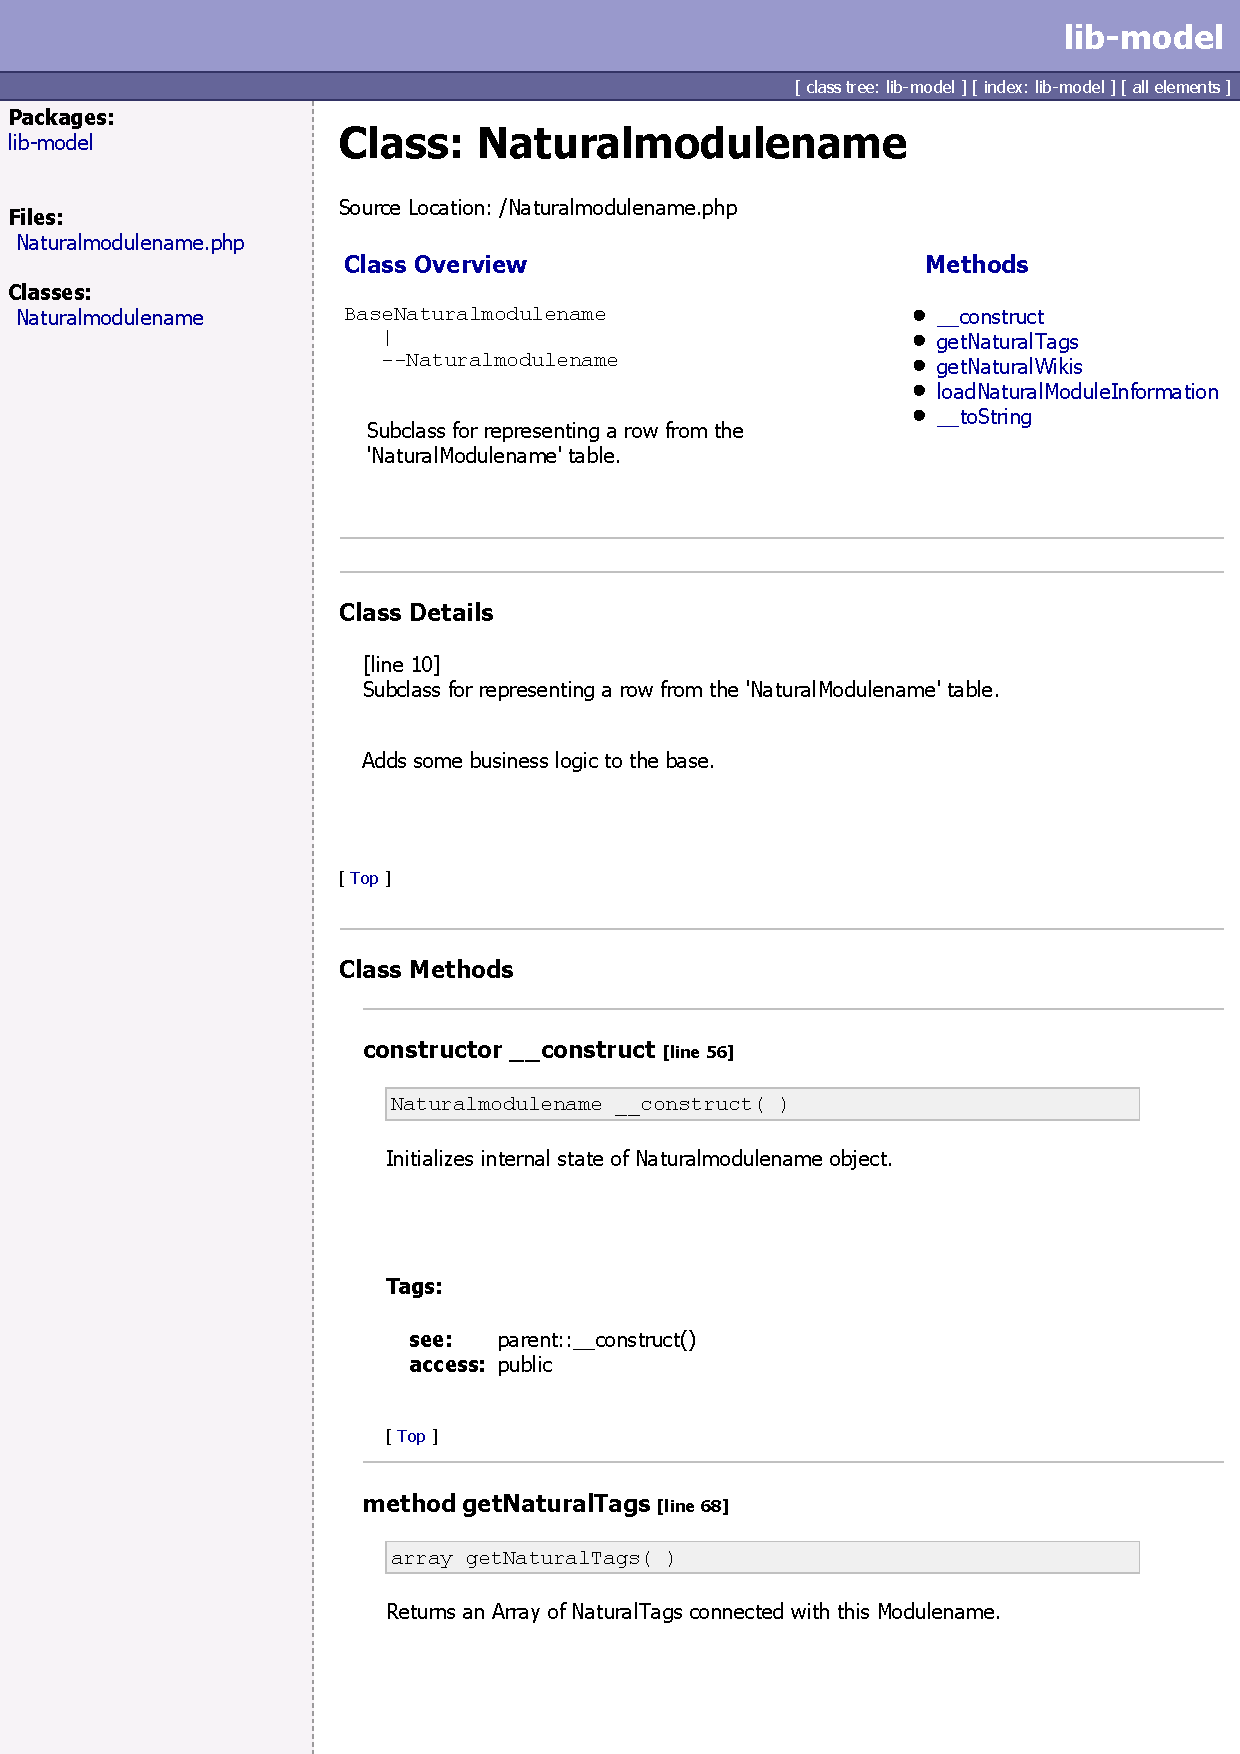
\includegraphics[page=1, width=0.9\textwidth]{doc.pdf}

\includegraphics[page=2, width=0.9\textwidth]{doc.pdf}
\end{center}

\clearpage
\subsection{Testfall und sein Aufruf auf der Konsole}
\label{app:Test}
\lstinputlisting[language=php, caption={Testfall in PHP}]{Listings/tests.php}
\clearpage
\begin{figure}[htb]
\centering
\includegraphicsKeepAspectRatio{testcase.jpg}{1}
\caption{Aufruf des Testfalls auf der Konsole}
\end{figure}


\subsection{Klasse: ComparedNaturalModuleInformation}
\label{app:CNMI}
Kommentare und simple Getter/Setter werden nicht angezeigt.
\lstinputlisting[language=php, caption={Klasse: ComparedNaturalModuleInformation}]{Listings/cnmi.php}
\clearpage

\subsection{Klassendiagramm}
\label{app:Klassendiagramm}
Klassendiagramme und weitere \acs{UML}-Diagramme kann man auch direkt mit \LaTeX{} zeichnen, siehe \zB \url{http://metauml.sourceforge.net/old/class-diagram.html}.
\begin{figure}[htb]
\centering
\includegraphicsKeepAspectRatio{Klassendiagramm.pdf}{1}
\caption{Klassendiagramm}
\end{figure}
\clearpage

\subsection{Benutzerdokumentation}
\label{app:BenutzerDoku}
Ausschnitt aus der Benutzerdokumentation:

\begin{table}[htb]
\begin{tabularx}{\textwidth}{cXX}
\rowcolor{heading}\textbf{Symbol} & \textbf{Bedeutung global} & \textbf{Bedeutung einzeln} \\
\includegraphicstotab[]{weather-clear.png} & Alle Module weisen den gleichen Stand auf. & Das Modul ist auf dem gleichen Stand wie das Modul auf der vorherigen Umgebung. \\
\rowcolor{odd}\includegraphicstotab[]{weather-clear-night.png} & Es existieren keine Module (fachlich nicht möglich). & Weder auf der aktuellen noch auf der vorherigen Umgebung sind Module angelegt. Es kann also auch nichts übertragen werden. \\
\includegraphicstotab[]{weather-few-clouds-night.png} & Ein Modul muss durch das Übertragen von der vorherigen Umgebung erstellt werden. & Das Modul der vorherigen Umgebung kann übertragen werden, auf dieser Umgebung ist noch kein Modul vorhanden. \\
\rowcolor{odd}\includegraphicstotab[]{weather-few-clouds.png} & Auf einer vorherigen Umgebung gibt es ein Modul, welches übertragen werden kann, um das nächste zu aktualisieren. & Das Modul der vorherigen Umgebung kann übertragen werden um dieses zu aktualisieren. \\
\includegraphicstotab[]{weather-storm.png} & Ein Modul auf einer Umgebung wurde entgegen des Entwicklungsprozesses gespeichert. & Das aktuelle Modul ist neuer als das Modul auf der vorherigen Umgebung oder die vorherige Umgebung wurde übersprungen. \\
\end{tabularx}
\end{table}




\end{document}
